% kapitel3.tex
\chapter{Algorithmus von Kezdy und McGuinness}
\label{cha:algorithmuskezdymcguinness}

Die Arbeit auf dem in \cite{KeM92} vorgestellten sequenziellen Algorithmus von Kezdy und McGuinness, der im Folgenden erklärt wird.
Als Eingabe wird ein ungerichteter Graph ohne Mehrfachkanten oder Schleifen erwartet, ausgegeben wird, ob der Graph einen $K_5$-Minor hat.
Für den Fall, dass einer gefunden wurde, kann zusätzlich ausgegeben werden, welche Knoten den Minor formen.
Die Laufzeit liegt in $\mathcal{O}(n^2)$. % TODO

Planaritätstests können bereits in linearer Laufzeit entscheiden, ob ein Graph einen \kf- oder \kdd-Minor enthält\cite{BoM04}.
Es muss folglich der Fall behandelt werden, in dem der Test stoppt, weil er einen \kdd-Minor gefunden hat.
Denn dann kann zunächst keine Aussage darüber getroffen werden, ob zusätzlich ein \kf-Minor enthalten ist.
Als Lösung bildet der Algorithmus von Kezdy und McGuinness in einem $3$-zusammenhängenden Graphen solange augmentierte Komponenten mit \dd-Separatoren, die Teil von \kdd-Minoren sein können, bis entweder alle Komponenten planar \bzw isomorph zu $W$ sind oder aber ein \kf-Minor gefunden wurde.


\section{Behandlung von \kdd-Minoren}
\label{sec:behandlung_von_kdd_minoren}

Die folgenden Theoreme, Lemmata und meisten Beweise sind \cite{KeM92} entnommen.

Um das zentrale Theorem aus \cite{KeM92}, welches den \kdd-Minor untersucht, zu erklären, wird zunächst die Gültigkeit augmentierter Komponenten behandelt:
\begin{theorem}[\cite{KeM92}]\label{eq:Theorem33}
  Für $k \geq 3$: Sei $G$ ein $k$-zusammenhängender Graph und $C$ ein $k$-Separator in $G$ mit $k \geq 3$.
  Jede durch $C$ definierte augmentierte Komponente ist ein Minor von $G$ \gdw es entweder mindestens $k$ Komponenten sind oder mindestens $k-1$, von denen mindestens zwei jeweils aus mehr als einem Knoten bestehen.
\end{theorem}
\begin{beweis}
  % Proof omitted in KeM92
  Seien $c_1, c_2, ..., c_k$ die Knoten von $C$ und $Z = \{Z_1, Z_2, ..., Z_k\}$ beziehungsweise $Z = \{Z_1, Z_2, ..., Z_{k-1}\}$ die Zusammenhangskomponenten, die durch $G - C$ entstehen.
  Die zugehörigen augmentierten Komponenten seien $A_1, A_2, ..., A_k$ \bzw $A_1, A_2, ..., A_{k-1}$.
  Betrachtet wird eine beliebige dieser augmentierten Komponenten $A_i$.
  Der Definition der augmentierten Komponenten nach finden sich bereits alle Knoten von $A_i$ in $G$ wieder. % Teilgraph
  Weiterhin enthält $G$ mindestens alle Kanten in $A_i - C$ sowie die verbindenden Kanten zwischen $A_i$ und $C$.
  Jedoch bilden in $A_i$ die Knoten von $C$ eine Clique, es existieren also \ggf Kanten zwischen den Knoten von $C$ in $A_i$, die es nicht in $G$ gibt.
  Es bleibt zu zeigen, dass die Kanten, die für diese Clique in $A_i$ nötig sind, durch Kantenkontraktionen in $G$ erzeugt werden können.
  Dadurch, dass $G$ $k$-zusammenhängend ist, besitzt jede Zusammenhangskomponente von $G - C$ Kanten zu allen $c_1, c_2, ..., c_k$.
  Würde eine Kante zu einem Knoten $c_j$ mit $1 \leq j \leq k$ fehlen, wäre ein $(k-1)$-Separator bestehend aus $C - c_j$ möglich, was im Widerspruch zu dem $k$-Zusammenhang stehen würde.
  Das Theorem unterscheided nun zwei Fälle, um die fehlenden Kanten bereitstellen zu können:
  \begin{enumerate}
    \item Es existieren $k$ Zusammenhangskomponenten.
          Wird $A_i$ betrachtet, kommen die Knoten in $Z - Z_i$ infrage, um durch Kantenkontraktionen die fehlenden Kanten für die Clique von $C$ in $A_i$ zu erzeugen.
          Um die Kanten von $C$ in $A_i$ in $G$ zu erzeugen, kann zunächst der Pfad, der $c_1$ mit $Z_1$ verbindet, kontrahiert werden.
          Anschließend ist $c_1$ mit allen Knoten in $C$ verbunden.
          Dies kann analog für alle Knoten in $C$ und den entsprechenden Zusammenhangskomponenten durchgeführt werden, außer für $c_i$, da $A_i$ der gesuchte Minor ist.
          Allerdings ist $c_i$ aufgrund des $k$-Zusammenhangs mit allen anderen Zusammenhangskomponenten verbunden, sodass $C$ nach den beschriebenen Kontraktionen eine Clique bildet.
    \item Es existieren $k-1$ Komponenten von denen mindestens zwei aus mehr als einem Knoten bestehen.
          Analog zum vorherigen Fall können die Pfade zwischen den Knoten von $C$ und den Zusammenhangskomponenten $A$ kontrahiert werden.
          Es fehlt jedoch ein Pfad, da eine Zusammenhangskomponente weniger vorliegt.
          Es gibt mindestens eine Zusammenhangskomponente aus $Z - Z_i$, die aus zwei oder mehr Knoten besteht.
          Da der Graph $k$-zusammenhängend ist, sind mindestens zwei dieser Knoten mit allen in $C$ verbunden, sodass sie durch Kontraktionen mit zwei unterschiedlichen Knoten aus $C$ genutzt werden können, um die gesuchte Clique zu erzeugen.
  \end{enumerate}
  Ein Beispiel, in dem die augmentierten Komponenten keine Minoren sind, findet sich in \Abb \ref{fig:Theorem33}.
\end{beweis}
\begin{figure}[H]
  \centering
  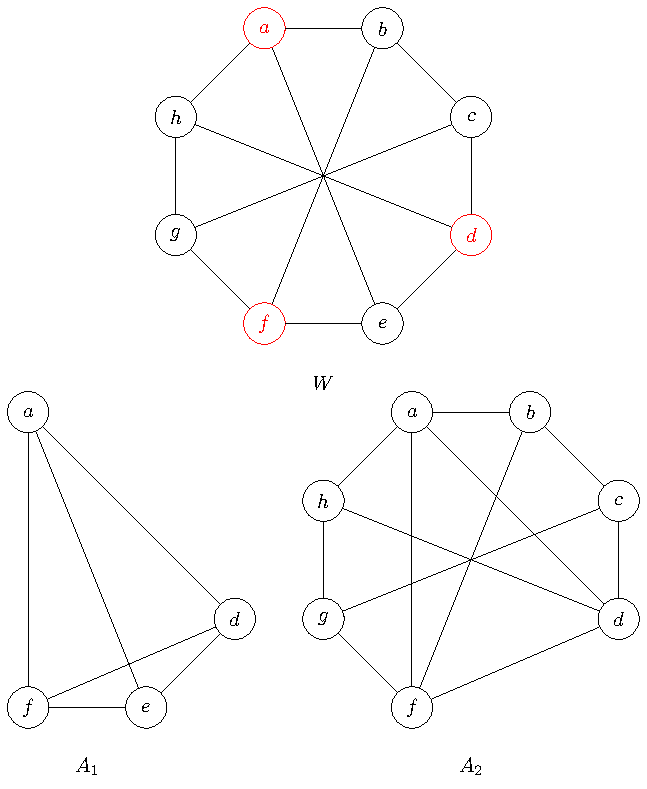
\includegraphics[keepaspectratio]{bilder/Theorem33.pdf}
  \caption{Gegenbeispiel zu Theorem \ref{eq:Theorem33} für  $k=3$ mit $C=\{a, d, f\}$ in $W$, wodurch die $k-1$ Komponenten $A_1$ und $A_2$ entstehen
           Es entstehen durch $W - C$ zwei Zusammenhangskomponenten, die die Knoten $\{e\}$ und $\{b, c, g, h\}$ enthalten.
           Entgegen der Voraussetzungen des Theorems gibt es daher nicht genügend Zusammenhangskomponenten \bzw keine zwei Zusammenhangskomponenten, die je mehr als zwei Knoten enthalten:
           Die Komponente $A_1$ ist zwar ein gültiger Minor, da sie etwa durch die Kontraktionen der Kanten $(a, b), (a, h), (f, g)$ und $(c, d)$ aus $W$ erzeugt werden kann.
           $A_2$ dagegen kann aber nicht durch Kontraktionen aus $W$ erzeugt werden -- wird beispielsweise die Kante $(d, e)$ in $W$ kontrahiert, fehlt die Kante $(a, f)$ in $A_2$.
           Analog kann $e$ mit keiner seiner inzidenten Kanten kontrahiert werden, um einen zu $A_2$ isomorphen Graphen zu erhalten.}
  \label{fig:Theorem33}
\end{figure}


Als nächstes stellen Kezdy und McGuinness fest, dass ein Graph in augmentierte Komponenten zerlegt werden kann, wenn ein \dd-Separators in ihm gefunden wurde:
\begin{theorem}[\cite{KeM92}]\label{eq:Theorem34}
  Sei $G$ ein $3$-zusammenhängender Graph mit einem \dd-Separator $C$.
  $G$ hat einen \kf-Minor \gdw eine der durch $C$ definierten augmentierten Komponenten einen \kf-Minor enthält.
\end{theorem}
\begin{beweis}[\cite{KeM92}]
  Zunächst kann festgestellt werden, dass, falls eine der augmentierten Komponenten einen \kf-Minor enthält, dieser laut Theorem \ref{eq:Theorem33} auch ein Minor von $G$ ist.
  Es bleibt zu zeigen, dass sich ein \kf-Minor nicht auf zwei augmentierte Komponenten erstreckt, sondern sich ausschließlich in einer befindet.
  Angenommen es gilt \kf \minor $G$ und zwei der Branch-Sets, die den \kf-Minor bilden, befinden sich jeweils vollständig in unterschiedlichen Zusammenhangskomponenten.
  In diesem Fall wäre $C$ ein $3$-Separator in dem gefundenen Minor, was im Widerspruch zu dem $4$-Zusammenhang des \kf steht.
\end{beweis}

Das zentrale Theorem ist darauf zurückzuführen, dass jeder Graph ohne \kf-Minor durch Cliquen-Summen von Teilgraphen, die planar oder isomorph zu $W$ sind, gebildet werden kann\cite{Wag37}.
Eine genauere Betrachtung findet in Kapitel \ref{cha:wagnerstruktur} statt.
Es kann benutzt werden, um einen Graph rekursiv in augmentierte Komponenten aufzuteilen, bis der Planaritätstest entweder einen \kf-Minor findet oder alle augmentierten Komponenten planar \bzw isomorph zu $W$ sind.
\begin{theorem}[\cite{KeM92}]\label{eq:Theorem36}
  Sei $G$ ein $3$-zusammenhängender Graph, der ein \kdd-Subdivision $S$ enthält, dessen Branch-Ends in die rote Knotenmenge $R = \{a, b, c\}$ und blaue $B = \{x, y, z\}$ unterteilt sind.
  Mindestens eine der folgenden Bedingungen trifft auf $G$ zu:
  \begin{enumerate}
    \item $G$ enthält einen \kf-Minor.\label{eq:Theorem361}
    \item $G$ ist isomorph zu $W$.\label{eq:Theorem362}
    \item $\{a, b, c\}$ bilden einen $3$-Separator, sodass $\{x, y, z\}$ in separaten Komponenten liegen.\label{eq:Theorem363}
    \item $\{x, y, z\}$ bilden einen $3$-Separator, sodass $\{a, b, c\}$ in separaten Komponenten liegen.\label{eq:Theorem364}
  \end{enumerate}
\end{theorem}
Durch die Theoreme \ref{eq:Theorem33} und \ref{eq:Theorem34} wurde gezeigt, dass der Graph in den Fällen \ref{eq:Theorem363} und \ref{eq:Theorem364} in augmentierte Komponenten zerlegt und darauf ein Planaritätstest ausgeführt werden kann.
Anschließend stellen die Autoren einige Lemmata auf, mit denen untersucht wird, ob $S$ einen \kf-Minor enthält -- also ob Bedingung \ref{eq:Theorem361} zutrifft.

\begin{lemma}[\cite{KeM92}]\label{eq:Lemma32}
  Sei $G$ ein $3$-zusammenhängender Graph und $S$ ein \kdd-Subdivision in $G$.
  Enthält $G$ drei Pfade von einem Knoten $w \in G - S$ zu drei nicht im selben Branch-Fan liegenden Knoten in $S$, enthält $G$ einen \kf-Minor.
\end{lemma}
\begin{beweis}[\cite{KeM92}]
  Seien $t, u, v$ die drei Endpunkte der Pfade in $S$.
  Mindestens einer von ihnen ist ein innerer Knoten, da sonst alle im selben Branch-Fan liegen würden.
  Sei \oBdA $t$ ein solcher innerer Knoten auf dem Pfad $P(a, x)$.
  Folglich können $u$ und $v$ nicht beide in $F(a)$ oder $F(x)$ liegen, sonst lägen alle drei im gleichen Branch-Fan.
  Es wird unterschieden, wo genau die drei Knoten in $S$ liegen -- die Fälle sind in den Abbildungen \ref{fig:Lemma321}, \ref{fig:Lemma322} und \ref{fig:Lemma323} skizziert.
  \begin{enumerate}
    \item $u$ und $v$ sind nicht im gleichen Branch-Fan wie $t$. \label{eq:Lemma321}
          Dann müssen $u$ und $v$ ebenfalls innere Knoten sein, im Beispiel auf den Pfaden $P(y, b)$ \bzw $P(z, c)$.
          Es kann ein $M$-Minor durch folgende Kontraktionen erzeugt werden: $u$ mit einem der roten und $v$ mit einem der blauen Knoten (analog $u$ mit blau und $v$ mit rot) sowie $P(w, t)$.
    \item $u$ oder $v$ liegen auf $P(a, x)$. \label{eq:Lemma322}
          Sei \oBdA $u \in P(a, x)$.
          Da $t$ ebenfalls in diesem Pfad liegt, gilt $\{t, u\} \in F(a) \cup F(x)$, sodass $v$ nicht in diesen beiden Branch-Fans liegen kann.
          Es können $t$ und $v$ getauscht werden, sodass eine Reduktion auf Fall \ref{eq:Lemma321} erreicht wird.
    \item Entweder $u$ oder $v$ liegen im gleichen Branch-Fan wie $t$. \label{eq:Lemma323}
          Sei \oBdA $u \in F(x) - P(a, x)$, im Beispiel auf dem Pfad $P(b, x)$.
          Es gilt $\{t, u\} \in F(x)$, weshalb $v$ in einem anderen Branch Fan sein muss.
          Da alle roten Knoten in $F(x)$ liegen, gilt konkreter $v \in (F(y) \cup F(z)) - \{a, b, c\}$
          Es können $P(b, u)$ kontrahiert werden sowie je nach Fall entweder $P(v, y)$ oder $P(v, z)$.
          Wird $P(w, t)$ ebenfalls kontrahiert, entsteht erneut ein $M$-Minor.
  \end{enumerate}
\end{beweis}
\begin{figure}[H]
  \centering
  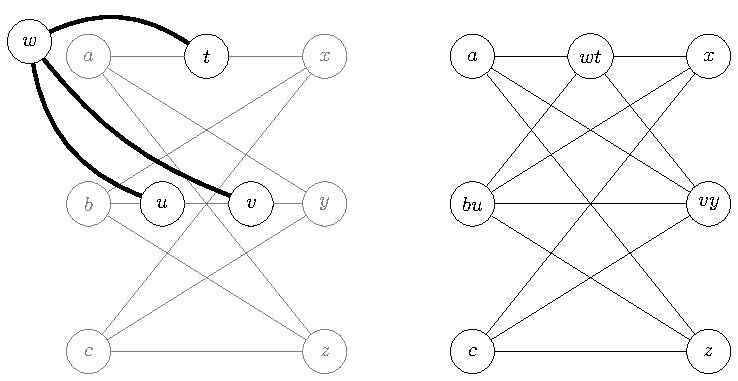
\includegraphics[keepaspectratio]{bilder/Lemma321.pdf}
  \caption{Beispiel zum ersten Fall von Lemma \ref{eq:Lemma32}.}
  \label{fig:Lemma321}
\end{figure}
\begin{figure}[H]
  \centering
  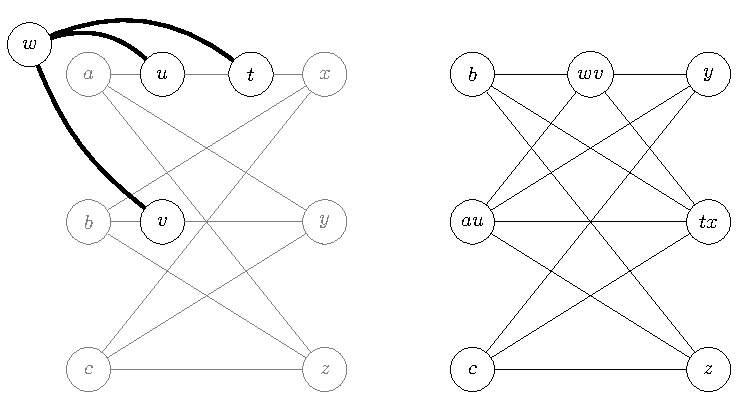
\includegraphics[keepaspectratio]{bilder/Lemma322.pdf}
  \caption{Beispiel zum zweiten Fall von Lemma \ref{eq:Lemma32}.}
  \label{fig:Lemma322}
\end{figure}
\begin{figure}[H]
  \centering
  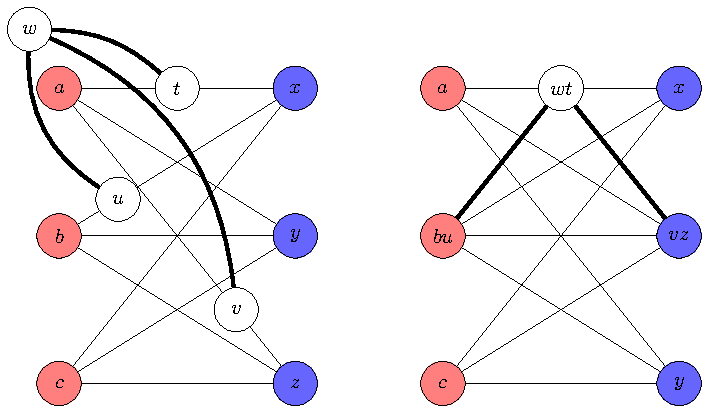
\includegraphics[keepaspectratio]{bilder/Lemma323.pdf}
  \caption{Beispiel zum dritten Fall von Lemma \ref{eq:Lemma32}.}
  \label{fig:Lemma323}
\end{figure}

\begin{lemma}[\cite{KeM92}]\label{eq:Lemma33}
  Sei $G$ ein $3$-zusammenhängender Graph und $S$ ein \kdd-Subdivision in $G$.
  Betrachtet wird ein Pfad außerhalb von $S$, der zwei Endpunkte hat, die in einem roten Branch-Fan, aber nicht im gleichen Branch-Path liegen.
  Analog dazu wird ein Pfad außerhalb von $S$ gesucht, dessen Endpunkte in einem blauen Branch-Fan liegen, ohne dass diese auf dem gleichen Branch-Path in $S$ liegen.
  Existieren diese beiden Pfade in $G$, dann enthält $G$ einen \kf-Minor.
\end{lemma}
\begin{beweis}[\cite{KeM92}]
  Sei $P_1$ der Pfad, der zwei Knoten in einem roten Branch-Fan verbindet und $P_2$ der, der zwei in einem blauen Branch-Fan verbindet.
  \OBdA hat $P_1$ Endpunkte in $F(a)$ und $P_2$ in $F(x)$.
  Da laut Bedingung die Endpunkte nicht in einem einzelnen Pfad von $S$ liegen, kann $a$ kein Endpunkt von $P_1$ und $x$ kein Endpunkt von $P_2$ sein.
  Es ergeben sich zwei Fälle:
  \begin{enumerate}
    \item Die beiden Pfade haben keine gemeinsamen Knoten.
          Da $P_1$ beide Endpunkte in $F(a)$ hat, liegen diese beiden Endpunkte in zwei unterschiedlichen blauen Branch-Fans.
          Entsprechend sind die Endpunkte von $P_2$ in unterschiedlichen roten Branch-Fans.
          Werden die Endpunkte von $P_1$ je mit den beiden blauen und die von $P_2$ mit den beiden roten Knoten von $S$ kontrahiert, entsteht ein \kf-Minor.
          \Abb \ref{fig:Lemma331} skizziert den Fall beispielhaft.
    \item Die beiden Pfade haben einen gemeinsamen Knoten $w$.
          Liegt dieser gemeinsame Knoten außerhalb von $S$, kann Lemma \ref{eq:Lemma32} angewendet werden, da die Endpunkte der Pfade nicht alle im gleichen Branch-Fan liegen.
          Liegt $w$ innerhalb von $S$, ist er ein Endpunkt von $P_1$ und $P_2$ und muss auf dem Pfad $P(a, x)$ liegen, da dieser der einzige gemeinsame Pfad ist, siehe links in \ref{fig:Lemma332}.
          Sei $P_1 = P(w, u)$ und $P_2 = P(w, v)$.
          Da $u$ nicht in $F(x)$ liegt und $v$ nicht in $F(a)$, gibt es einen Pfad von $u$ zu einem blauen Knoten und von $v$ zu einem roten Knoten, die sich nicht kreuzen und daher kontrahiert werden können.
          Durch die Kontraktion dieser beiden Pfade entsteht, wie in \Abb \ref{fig:Lemma332} rechts zu sehen, ein $M$-Minor.
  \end{enumerate}
\end{beweis}
\begin{figure}[H]
  \centering
  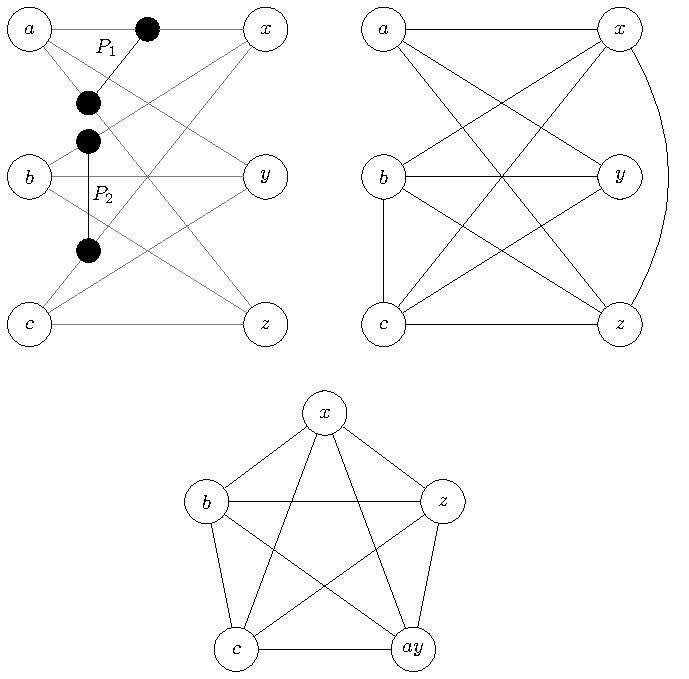
\includegraphics[keepaspectratio]{bilder/Lemma331.pdf}
  \caption{Beispiel zum ersten Fall von Lemma \ref{eq:Lemma33}.
           Links oben ist $S$ mit zwei zusätzlichen Pfaden aus $G$ abgebildet.
           $P_1$ hat beide Endpunkte in $F(a)$ sowie den blauen Branch-Fans $F(x)$ und $F(y)$, mit denen die Endpunkte kontrahiert werden.
           $P_2$ hat seine Endpunkte in den roten Branch-Fans $F(b)$ und $F(c)$, mit denen sie kontrahiert werden.
           Rechts oben ist der dadurch entstehende Minor abgebildet und unten wird der enthaltene \kf-Minor gezeigt.}
  \label{fig:Lemma331}
\end{figure}
\begin{figure}[H]
  \centering
  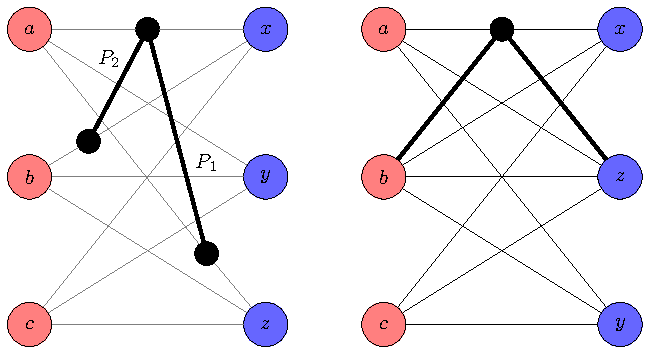
\includegraphics[keepaspectratio]{bilder/Lemma332.pdf}
  \caption{Beispiel zum zweiten Fall von Lemma \ref{eq:Lemma33}.
           Rechts ist der enthaltene $M$-Minor abgebildet.}
  \label{fig:Lemma332}
\end{figure}

\begin{lemma}[\cite{KeM92}]\label{eq:Lemma34}
  Sei $G$ ein $3$-zusammenhängender Graph und $S$ ein \kdd-Subdivision in $G$.
  Betrachtet wird ein Pfad außerhalb von $S$, der zwei innere Knoten paralleler Pfade in $S$ verbindet, sowie ein Pfad außerhalb von $S$, dessen Endpunkte nicht beide im gleichen Pfad von $S$ liegen.
  Bestehen die Endpunkte der beiden Pfade aus mindestens drei unterschiedlichen Knoten in $S$, enthält $G$ einen \kf-Minor.
\end{lemma}
% TODO Beweis

\begin{lemma}[\cite{KeM92}]\label{eq:Lemma35}
  Sei $G$ ein $3$-zusammenhängender Graph und $S$ ein \kdd-Subdivision in $G$ mit den roten Knoten $R = \{a, b, c\}$ und den blauen Knoten $B = \{x, y, z\}$.
  Bilden weder $R$ noch $B$ einen $3$-Separator, enthält $G$ einen \kf-Minor.
\end{lemma}
\begin{beweis}[\cite{KeM92}]
  Falls $R$ und $B$ keinen \dd-Separator bilden, ist sowohl der Graph $G - R$ als auch $G - B$ zusammenhängend.
  Sei $P_1$ ein Pfad, der zwei blaue Branch-Fans in $G - R$ und $P_2$ einer, der zwei rote Branch-Fans in $G - B$ verbindet.
  Beide liegen außerhalb von $S$.
  Die Endpunkte von $P_1$ seien $u_1$ und $v_1$, die von $P_2$ seien $u_2$ und $v_2$.
  $u_1$ und $v_1$ besitzen jeweils einen Pfad in $S$ zu einem der roten Knoten.
  Folglich gibt es einen dritten roten Knoten, der keinen solchen Pfad besitzt -- $u_2$ wird so gewählt, dass er in dem Branch-Fan dieses Knotens liegt.
  Demnach sind $u_1$, $v_1$ und $u_2$ unterschiedliche Knoten.
  Anschließend kann je nach vorliegendem Fall die Aussage auf eines der vorherigen Lemmata reduziert werden:
  \begin{enumerate}
    \item $P_1$ oder $P_2$ verbindet zwei parallele Pfade in $S$.
          In dem Fall kann Lemma \ref{eq:Lemma34} angewendet werden und $G$ enthält einen \kf-Minor.
    \item Die Endpunkte von $P_1$ liegen in einem einzelnen roten Branch-Fan -- analog liegen die von $P_2$ in einem blauen.
          Nach Lemma \ref{eq:Lemma33} enthält $G$ einen \kf-Minor.
  \end{enumerate}
\end{beweis}

\begin{figure}{H}
  \centering
  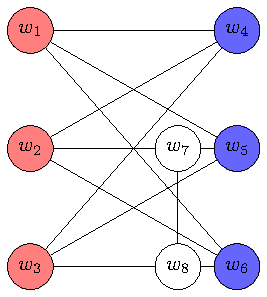
\includegraphics[keepaspectratio]{bilder/W2.pdf}
  \caption{Darstellung von einem Graph $S$, der isomorph zu $W$ ist.}
  \label{fig:W2}
\end{figure}
\begin{lemma}[\cite{KeM92}]\label{eq:Lemma36}
  Sei $G$ ein $3$-zusammenhängender Graph mit einer $W$-Subdivision.
  Ist $G$ nicht isomorph zu $W$, enthält $G$ einen \kf-Minor.
\end{lemma}
\begin{beweis}
  % Proof omitted in KeM92
  $G$ enthält mindestens acht Knoten, die $S$ formen.
  Sei $G = (V_G, E_G)$ der Graph und $S = (V_S, E_S)$ der Teilgraph mit $V_S \subseteq V_G$ und $E_S \subseteq E_G$, der die $W$-Subdivision formt.
  Da $W$ keinen \kf-Minor enthält, besitzt jeder Graph, der isomorph zu $W$ ist, ebenfalls keinen.
  Es wird deshalb angenommen, dass $G$ nicht isomorph zu $W$ ist.
  Damit $G$ nicht isomorph zu $W$ ist trifft mindestens einer der Punkte auf $G$ zu:
  \begin{enumerate}
    \item Es gibt eine weitere Kante $e = (w_i, w_j) \in E_G$ mit $\{w_i, w_j\} \in V_S$, aber $e \notin E_G$.
    Seien die Knoten $w_1, ..., w_8 \in V_S$ \oBdA so gewählt, wie in \Abb \ref{fig:W2} gezeigt.
    Seien $R = \{w_1, w_2, w_3\}$ als rote und $B = \{w_4, w_5, w_6\}$ als blaue Knoten bezeichnet.
    $R$ bildet keinen \dd-Separator in $S$, da es den Pfad $P(w_5, w_6)$ in $S - R$ gibt.
    Analog ist $B$ kein \dd-Separator wegen dem Pfad $P(w_2, w_3) \in S - B$.
    Verbindet die zusätzliche Kante zwei Knoten in $R$, dann ist $e$ eine Kante, deren Endpunkte in einem blauen Branch-Fan, aber nicht auf dem gleichen Branch-Path liegen.
    Außerdem gibt es durch den Pfad $P(w_5, w_6)$ eine Kante, die zwei Endpunkte in einem roten Branch-Fan verbindet, die nicht auf dem gleichen Branch-Path liegen.
    Das Problem kann zu Lemma \ref{eq:Lemma33} reduziert werden (erster Fall von \ref{eq:Lemma33}).
    Die Reduktion kann analog für $P(w_2, w_3)$ angewendet werden, wenn $e$ zwei blaue Knoten verbindet.
    Übrig bleibt der Fall, dass ein Endpunkt von $e$ entweder $w_7$ oder $w_8$ ist und der andere Endpunkt einer der roten oder einer der blauen Knoten ist.
    Sei \oBdA $e = (w_1, w_7)$.
    Dann liegen die Endpunkte von $e$ in einem blauen Branch-Fan ($F(w_5)$), aber nicht dem gleichen Branch-Path.
    Außerdem verbinden die Endpunkte der Kante $(w_7, w_8)$ zwei parallele Branch-Paths ($P(w_2, w_5)$ und $P(w_3, w_6)$).
    Damit kann der Fall zu Lemma \ref{eq:Lemma34} reduziert werden.
    \item Es gibt einen weiteren Knoten $v \in V_G$ mit $v \notin V_S$.
    Er hat aufgrund des $3$-Zusammenhangs mindestens drei Pfade zu Knoten von $S$.
    Seien diese drei Knoten $\{w_1, w_2, w_3\} \in V_S$ beliebig.
    Da es in $W$ keine Cliquen der Größe $3$ gibt, sind mindestens zwei der drei Knoten nicht adjazent.
    Sei \oBdA $e = (w_1, w_2) \notin E_S$.
    Da $\{(w_1, v), (v, w_2)\} \in E_G$ gilt, kann eine dieser beiden Kanten kontrahiert werden, sodass durch die jeweils andere $w_1$ und $w_2$ adjazent sind.
    Der Minor $S'$ mit $E_S' \cup e$ für $e = (w_1, w_2)$ kann auf den vorherigen Fall reduziert werden, da eine Kante außerhalb von $S$ gefunden wurde.
  \end{enumerate}
\end{beweis}

Als nächstes folgt der Beweis zu \ref{eq:Theorem36}.
\begin{beweis}[\cite{KeM92}]
  Gezeigt wird, dass, falls $S$ keinen \dd-Separator bildet, $G$ entweder einen \kf-Minor enthält oder isomorph zu $W$ ist.
  Falls kein \kf-Minor enthalten ist, gilt nach Lemma \ref{eq:Lemma35}, dass $G - R$ oder $G - B$ nicht zusammenhängend ist.
  Demnach ist $B$ ein $3$-Separator, der den Graph teilt, aber die Knoten aus $R$ liegen nicht alle in unterschiedlichen Zusammenhangskomponenten.
  Deshalb muss es außerhalb von $S$ mindestens einen Pfad $P_1$ geben, der zwei der roten Knoten in $G - B$ verbindet.
  Analog gibt es einen Pfad $P_2$, der zwei blaue Knoten in $G - R$ verbindet.
  Da $P_1$ zwei rote Branch-Fans verbindet, liegen seine Endpunkte in zwei verschiedenen Pfaden von $S$.
  Gleiches gilt für die Endpunkte von $P_2$.
  Liegen die Endpunkte von $P_1$ beide in einem einzelnen blauen Branch-Fan und die von $P_2$ in einem einzelnen roten, dann enthält $G$ laut Lemma \ref{eq:Lemma33} einen \kf-Minor.
  Liegen die Endpunkte von $P_1$ in parallelen Pfaden von $S$, enthält $G$ laut Lemma \ref{eq:Lemma34} einen \kf-Minor, da die Endpunkte von $P_2$ nicht auf einem Pfad von $S$ liegen (analog falls $P_2$ auf parallelen Pfaden liegt).
  Übrig bleibt die Möglichkeit, dass die Endpunkte der beiden Pfade paarweise identisch sind, siehe $P(w_7, w_8)$ in \Abb \ref{fig:W2}.
  Dann ist $G$ ein Subdivision zu $W$ und enthält laut Lemma \ref{eq:Lemma36} keinen \kf-Minor bei Isomorphie zu $W$.
\end{beweis}


\section{Sequenzieller Algorithmus zum Finden von \kf-Minoren}
\label{sec:sequenzieller_algorithmus_zum_finden_von_kf_minoren}

Da die Theoreme größtenteils auf $3$-zusammenhängenden Graphen arbeiten, muss der Eingabegraph \ggf zunächst angepasst werden, bevor der Planaritätstests angewendet werden kann.
Ist der Graph $1$-zusammenhängend, gibt es einen Knoten, der einen $(1, j)$-Separator für $j \geq 2$ bildet.
Genauso müssen zwei Knoten existieren, die einen $(2, j)$-Separator bilden, falls der Graph $2$-zusammenhängend ist.
In beiden Fällen kann der Separator benutzt werden, um den Graphen in $j$ augmentierte Komponenten zu zerlegen.
Anschließend kann der $3$-Zusammenhang der einzelnen Komponenten rekursiv geprüft werden.
Sind die Komponenten alle $3$-zusammenhängend, kann auf jede ein Planaritätstest angewendet werden.
Kezdy und McGuinness verwenden den Williamson-Algorithmus\cite{Wil84}, welcher in Linearzeit für einen Graphen einen \kf- \bzw \kdd-Subdivision ausgibt oder feststellt, dass der Graph planar ist.
In der Implementierung wird stattdessen der Planaritätstest von Boyer und Myrvold\cite{BoM04} verwendet, der bereits in \OGDF existiert.
Ergibt der Planaritätstest, dass eine Komponente planar ist, wird sie nicht weiter beachtet.
Enthält sie einen \kf-Minor, kann der Algorithmus stoppen und diesen ausgeben.
Wird ein \kdd-Minor gefunden, wird geprüft, welcher der vier Fälle aus Theorem \ref{eq:Theorem36} zutrifft.
Bei Isomorphie zu $W$ wird die Komponente nicht weiter beachtet.
Ist der \kdd-Minor ein \dd-Separator in der untersuchten Komponente, kann sie in weitere augmentierte Komponenten zerlegt und der Algorithmus rekursiv darauf angewendet werden.
Andernfalls müssen genügend Pfade in der Komponente existieren, sodass der \kdd-Minor auch einen \kf-Minor bildet und der Algorithmus ihn ausgeben und anhalten kann.
Diese Schritte werden solange wiederholt, bis alle augmentierten Komponenten planar \bzw isomorph zu $W$ sind oder ein \kf-Minor gefunden wurde.

\newpage
Für einen Graphen $G$ sind die einzelnen Schritte zusammengefasst:
\begin{enumerate}
  \item \label{item:algorithmus11} Gibt es einen $1$-Separator in $G$, dann bilde damit augmentierte Komponenten und wende den Algorithmus rekursiv auf jede an.
  \item \label{item:algorithmus12} Gibt es einen $2$-Separator in $G$, dann bilde damit augmentierte Komponenten und wende den Algorithmus rekursiv auf jede an.
  \item \label{item:algorithmus13} Planaritätstest:
                                   \begin{enumerate}
                                     \item $G$ ist planar: Gib zurück, dass kein \kf-Minor gefunden wurde.
                                     \item $G$ enthält ein \kf-Subdivision: Gib den \kf-Minor zurück und beende den Algorithmus.
                                     \item $G$ enthält ein \kdd-Subdivision: Weiter zu Schritt \ref{item:algorithmus14}
                                   \end{enumerate}
  \item \label{item:algorithmus14} $G$ ist isomorph zu $W$: Gib zurück, dass kein \kf-Minor gefunden wurde.
                                   $G$ ist nicht isomorph zu $W$: Weiter zu Schritt \ref{item:algorithmus15}
  \item \label{item:algorithmus15} Seien $R = \{a, b, c\}$ die roten und $B = \{x, y, z\}$ die blauen Branch-Ends der \kdd-Subdivision.
                                   Ist $R$ einen \dd-Separator, sodass alle Knoten aus $B$ in unterschiedlichen Zusammenhangskomponenten sind, dann bilde damit augmentierte Komponenten und wende den Algorithmus rekursiv auf jede an.
                                   (Analog für $B$ als Separator)
  \item \label{item:algorithmus16} Ist dieser Schritt erreicht, enthält $G$ einen \kf-Minor bestehend aus der \kdd-Subdivision, dem Pfad, der zwei rote, sowie dem Pfad, der zwei blaue Knoten verbindet.
\end{enumerate}
